\input{../preamble.tex}

\SetDate[10/03/2026]
\reversemarginpar
\setlength{\marginparsep}{.5cm}

\begin{document}
\pagestyle{fancy}
\fancyhead[L]{Seconde}
\fancyhead[C]{\textbf{Évaluation blanche — Probabilités}}
\fancyhead[R]{\today}

\null\vspace{-20pt}
Consignes particulières : 
\begin{itemize}[label=$\bullet$]
	\item 
	La calculatrice est {autorisée}.
	\item
	Sauf mention du contraire, toutes les réponses doivent être justifiées.
	%\item
	%L'exercice \ref{exe:prop-fond} peut être entièrement fait sur la feuille d'évaluation.
	\item
	L'évaluation fait \pageref{lastpage} page. La somme des points est \total{points}.
\end{itemize}

\marginpar{[pts]}
\hrule



\exe{6}{
	On tire un boule dans une urne contenant 3 boules bleues et 4 boules vertes.
	\begin{enumerate}[label=$\bullet$]
		\item Si la boule tirée est verte, on jette un dé équilibré à 3 faces (1 à 3).
		\item Si la boule tirée est bleue, on jette un dé équilibré à 6 faces (1 à 6).
	\end{enumerate}

	Créer un arbre de probabilité pour cette situation et répondre aux questions suivantes. Donner les probabilités sous forme de fraction irréductible.
	\begin{enumerate}
		\item Quelle est la probabilité d'obtenir un nombre pair ?
		\item Quelle est la probabilité d'obtenir un multiple de $3$ ?
		\item Quelle est la probabilité d'obtenir un nombre pair \textbf{ou} un multiple de $3$ ?
		\item Calculer la probabilité d'obtenir $6$.
		\item Énoncer le principe d'inclusion-exclusion et le vérifier.
	\end{enumerate}

}{exe:exe14}{
	On a l'arbre suivant.
	
	\begin{center}
	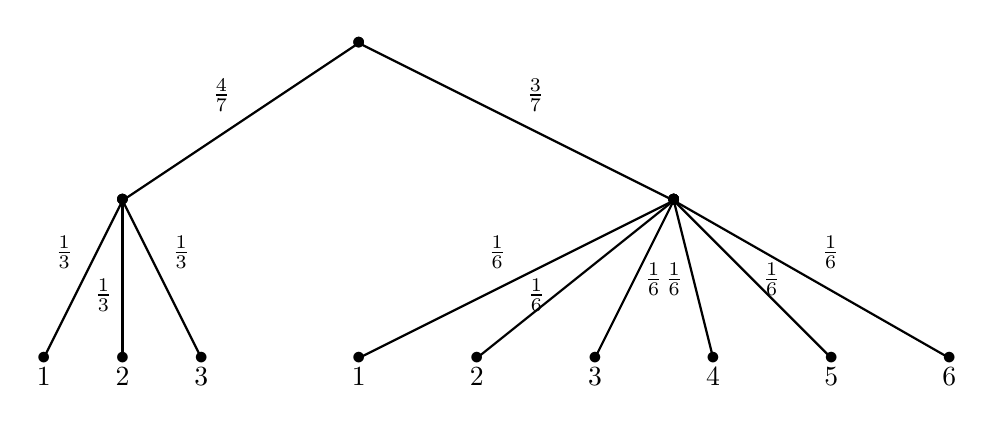
\begin{tikzpicture}
		% depth 1
		\draw[-, thick, black] (0,0) node {$\bullet$} -- (4,-2) node[midway, above right] {$\frac37$};
		\draw[-, thick, black] (0,0) node {$\bullet$} -- (-3,-2) node[midway, above left] {$\frac47$};
		% depth 2
		% gauche -> droite
		% verte
		\draw[-, thick, black] (-3,-2) node {$\bullet$} -- (-2,-4) node[midway, above right] {$\frac13$};
		\draw[-, thick, black] (-3,-2) node {$\bullet$} -- (-3,-4) node[pos=.6, left] {$\frac13$};
		\draw[-, thick, black] (-3,-2) node {$\bullet$} -- (-4,-4) node[midway, above left] {$\frac13$};
		
		\draw (-4,-4) node {$\bullet$};
		\draw (-3,-4) node {$\bullet$};
		\draw (-2,-4) node {$\bullet$};
		\draw (-4,-4) node[below] {$1$};
		\draw (-3,-4) node[below] {$2$};
		\draw (-2,-4) node[below] {$3$};
		
		% bleue
		\draw[-, thick, black] (4,-2) node {$\bullet$} -- (0,-4) node[midway, above left] {$\frac16$};
		\draw[-, thick, black] (4,-2) node {$\bullet$} -- (1.5,-4) node[pos=.6, left] {$\frac16$};
		\draw[-, thick, black] (4,-2) node {$\bullet$} -- (3,-4) node[midway, right] {$\frac16$};
		\draw[-, thick, black] (4,-2) node {$\bullet$} -- (4.5,-4) node[midway, left] {$\frac16$};
		\draw[-, thick, black] (4,-2) node {$\bullet$} -- (6,-4) node[midway, right] {$\frac16$};
		\draw[-, thick, black] (4,-2) node {$\bullet$} -- (7.5,-4) node[midway, above right] {$\frac16$};
		
		\draw (0,-4) node {$\bullet$};
		\draw (1.5,-4) node {$\bullet$};
		\draw (3,-4) node {$\bullet$};
		\draw (4.5,-4) node {$\bullet$};
		\draw (6,-4) node {$\bullet$};
		\draw (7.5,-4) node {$\bullet$};
		\draw (0,-4) node[below] {$1$};
		\draw (1.5,-4) node[below] {$2$};
		\draw (3,-4) node[below] {$3$};
		\draw (4.5,-4) node[below] {$4$};
		\draw (6,-4) node[below] {$5$};
		\draw (7.5,-4) node[below] {$6$};
		
	\end{tikzpicture}
	\end{center}
	
	\begin{enumerate}
		\item
			\begin{align*}
				P(\text{« nombre pair »}) &= P(2) + P(4) + P(6) \\
					&= \left( \frac47 \times \frac13 + \frac37\times\frac16 \right) + \left( \frac37 \times \frac16 \right) + \left( \frac37 \times \frac16 \right) \\
					&= \frac4{21} + \frac1{14} + \frac1{14} + \frac1{14} \\
					&= \frac{17}{42}.
			\end{align*}
		\item
			\begin{align*}
				P(\text{« multiple de $3$ »}) &= P(3) + P(6) \\
					&= \left( \frac47 \times \frac13 + \frac37\times\frac16 \right) + \left( \frac37 \times \frac16 \right) \\
					&= \frac4{21} + \frac1{14} + \frac1{14} \\
					&= \frac13.
			\end{align*}
		\item
			\begin{align*}
				P(\text{« multiple de $3$ ou de $2$ »}) &= P(2) + P(3) + P(4) + P(6) \\
					&= \left( \frac47 \times \frac13 + \frac37\times\frac16 \right) + \left( \frac47 \times \frac13 + \frac37\times\frac16 \right) + \left( \frac37 \times \frac16 \right) + \left( \frac37 \times \frac16 \right) \\
					&= \frac4{21} + \frac1{14} + \frac4{21} + \frac1{14} + \frac1{14} + \frac1{14} \\
					&= \frac23.
			\end{align*}
		\item 
			\begin{align*}
				P(6) &=\left( \frac37 \times \frac16 \right) \\
					&= \frac1{14}.
			\end{align*}
		
		\item
		On vérifie l'inclusion-exclusion en comparant $P(\text{« multiple de $3$ ou de $2$ »})$ et $P(\text{« multiple de $3$ »}) + P(\text{« multiple de $2$ »}) - P(6)$.
		D'une part,
			\[ P(\text{« multiple de $3$ ou de $2$ »}) = \frac23, \]
		et d'autre part,
			\begin{align*}
				P(\text{« multiple de $3$ »}) + P(\text{« multiple de $2$ »}) - P(6) &= \frac13 + \frac{17}{42} - \frac1{14} \\
				&= \frac{14 + 17 - 3}{42} \\
				&= \frac{28}{42} = \frac23.
			\end{align*}
	\end{enumerate}
}

\exe{4}{
	L'univers associé à une expérience aléatoire est $\{ A, B, C\}$.
	La loi de probabilité $P$ est donnée par le tableau ci-dessous et dépend d'un réel $t\in\R$ encore inconnu.
	\begin{multicols}{2}
	\begin{enumerate}
		\item Développer le carré $\left(t-\dfrac35\right)^2$.
		\item Déterminer $t$.
		\item Compléter la dernière ligne du tableau.
	\end{enumerate}
	\end{multicols}
	\begin{center}
	\begin{tabular}{|c|c|c|c|} \hline
		Résultat & $A$ & $B$ & $C$ \\ \hline
		Probabilité & $\frac9{25}$ & $t^2$ & $-\frac65 t$ \\ \hline
		Probabilité ($t = \dots\dots$) & $\frac9{25}$ & & \\ \hline
	\end{tabular}
	\end{center}
}{exe:carre}{
	On développe le carré à l'aide de l'identité remarquable
		\[ (a-b)^2 = a^2 + b^2 - 2ab, \]
	où, ici, on a $a=t$ et $b=\frac12.$
		\begin{align*}
			\left(t-\dfrac12\right)^2 &= t^2 + \left(\dfrac12\right)^2 - 2 \cdot t \cdot \dfrac12 \\
									&= t^2 + \dfrac14 - t
		\end{align*}
	On cherche désormais le $t\in\R$ pour lequel $P$ est une loi de probabilité. 
	Un loi vérifie les deux propriétés suivantes :
		\begin{itemize}
			\item $P(\omega) \in [0;1]$ pour chaque issue $\omega \in \Omega$ ; et
			\item $P(\Omega) = 1$.
		\end{itemize}
	La deuxième identité donne donc
		\begin{align*}
			P(a) + P(b) + P(c) = 1 && \iff && t^2 - t + \dfrac14 = 1.
		\end{align*}
	Le carré développé nous permet d'écrire
		\[ \left(t-\dfrac12\right)^2 = 1, \]
	et donc
		\[ \left|t-\dfrac12\right| = \sqrt{1} = 1, \]
	en utilisant le fait que $\sqrt{x^2} = |x|.$
	L'expression à l'intérieur de la valeur absolue est donc soit $+1$, soit $-1$, et on a donc deux alternatives :
		\begin{align*}
			t-\dfrac12 = 1 && \text{ ou } && t - \dfrac12 = -1 \\
			t = \dfrac32 && \text{ ou } && t = -\dfrac12.
		\end{align*}
	Pour s'entraîner à ce genre de résolution, voir la feuille d'exercices Fonctions 3.
	
	Comme les probabilités sont des nombres entre $0$ et $1$, on peut écarter la première solution car $P(a) = t^2$ serait strictement supérieur à $1$, et $P(b) = -t$, serait strictement négatif.
	Il ne reste donc que $t = -\frac12$, qui donne le tableau de probabilités suivant.
	\begin{center}
	\begin{tabular}{|c|c|c|c|} \hline
		Issue & $a$ & $b$ & $c$ \\ \hline
		Probabilité & $\frac14$ & $\frac12$ & $\frac14$ \\ \hline
	\end{tabular}
	\end{center}
}



\exe{6}{
	On lance un grand nombre de fois un D6, dé à 6 faces.
	Les résultats sont décrits dans le tableau suivant.
	\begin{center}
	\begin{tabular}{|c|c|c|c|c|c|c|} \hline
		Face & 1 & 2 & 3 & 4 & 5 & 6 \\ \hline
		Nombre de tirages & 19699 & 27549 & 9097 & 22999 & 27989 & 6970  \\ \hline
		Fréquence & & & & & & \\ \hline
	\end{tabular}
	\end{center}
	
	\begin{enumerate}
		\item Compléter le tableau en arrondissant à $10^{-2}$.
		\item Modéliser la réalité en définissant un univers et une loi de probabilité associés à l'expérience aléatoire du lancer de dé.
		\item Quelle est la probabilité d'obtenir un multiple de $3$ ?
		\item Quelle est la probabilité d'obtenir exactement trois $1$ en quatre lancers consécutifs ?
		\item Quelle est la probabilité d'obtenir au moins un $3$ après dix lancers consécutifs ?
	\end{enumerate}
}{exe:3}{
	todo
}


\exe{4}{
	On considère un univers
		\[ \Omega = \bigset{ -3 ; -2 ; 1 ; 4; 5; 7 ; 13 }, \]
	ainsi que deux sous-ensembles 
		\begin{align*}
			A = \bigset{ -3 ; 1 ; 5 } && \et && B = \bigset{ 1 ; 4 ; 5 ; 7 }.
		\end{align*}
	\begin{enumerate}
		\item Donner $\overline{A}$, le complémentaire de $A$ dans l'univers $\Omega$.
		\item Vérifier l'égalité
			\[ |A\cup B| = |A| + |B| - |A\cap B| \]
		en calculant le membre de gauche et le membre de droite puis en comparant les valeurs obtenues.
	\end{enumerate}

}{exe:4}{
	\begin{enumerate}
		\item Le complémentaire de $A$ dans $\Omega$ correspond à l'ensemble $\overline{A}$ qui contient tous les éléments de $\Omega$ sauf ceux appartenant à $A$. On note aussi $\Omega \setminus A$ ou $\Omega - A$.
			\[ \overline{A} = \{ -2 ; 4; 7; 13 \}. \]
		\item Le cardinal d'un ensemble est égal au nombre d'éléments distincts lui appartenant.
			À gauche on calcule donc
				\[ |A \cup B| = | \{ -3 ; 1; 5 ;4 ; 7 \} | = 5. \]
			À droite on trouve
				\[ |A| + |B| - |A\cap B| = 3 + 4 - | \{ 1 ; 5 \} | = 3 + 4 - 2 =  5. \]
	\end{enumerate}

}

\exe{2, difficulty=1}{
	\begin{enumerate}
		\item
		Soit $\Omega = \{1 ; 2 ; 3 \}$.
		Combien de sous-ensembles $E \subseteq \Omega$ existe-t-il ?
		\item
		Soit $\Omega = \{1 ; 2 ; 3 ; \dots ; n-1 ; n \}$ dépendant d'un entier naturel $n\in\N$ non nul.
		Combien de sous-ensembles $E \subseteq \Omega$ existe-t-il ?
	\end{enumerate}´
}{exe:subset}{
	todo
}


%%%%%%%%%%%

\label{lastpage}
\newpage
\fancyhead[C]{\textbf{Solutions}}
\shipoutAnswer
	
\end{document}
